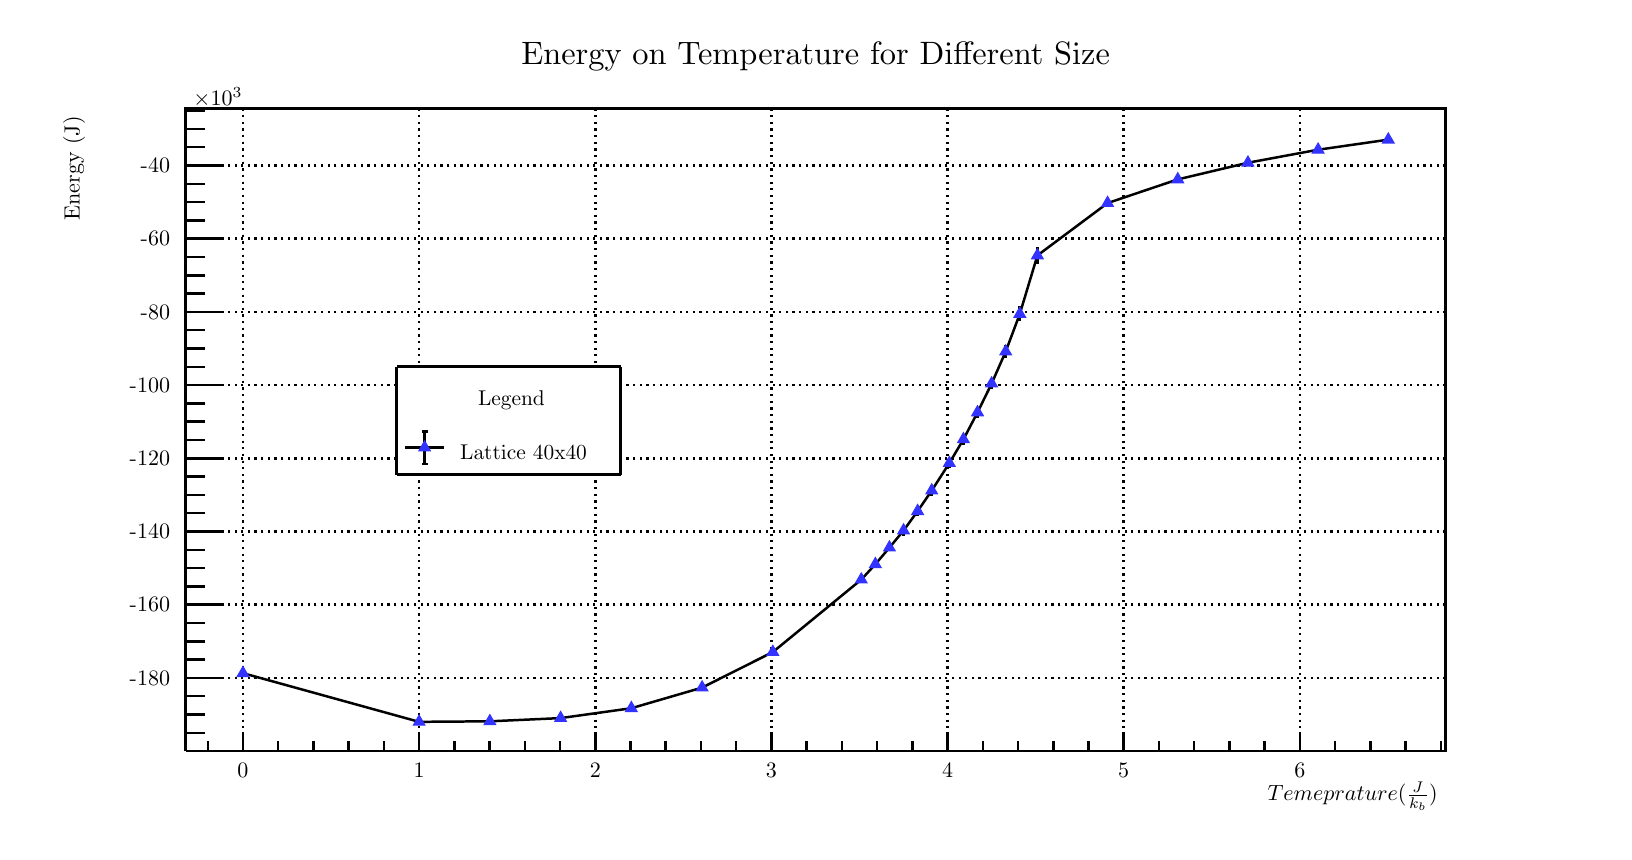
\begin{tikzpicture}
\pgfdeclareplotmark{cross} {
\pgfpathmoveto{\pgfpoint{-0.3\pgfplotmarksize}{\pgfplotmarksize}}
\pgfpathlineto{\pgfpoint{+0.3\pgfplotmarksize}{\pgfplotmarksize}}
\pgfpathlineto{\pgfpoint{+0.3\pgfplotmarksize}{0.3\pgfplotmarksize}}
\pgfpathlineto{\pgfpoint{+1\pgfplotmarksize}{0.3\pgfplotmarksize}}
\pgfpathlineto{\pgfpoint{+1\pgfplotmarksize}{-0.3\pgfplotmarksize}}
\pgfpathlineto{\pgfpoint{+0.3\pgfplotmarksize}{-0.3\pgfplotmarksize}}
\pgfpathlineto{\pgfpoint{+0.3\pgfplotmarksize}{-1.\pgfplotmarksize}}
\pgfpathlineto{\pgfpoint{-0.3\pgfplotmarksize}{-1.\pgfplotmarksize}}
\pgfpathlineto{\pgfpoint{-0.3\pgfplotmarksize}{-0.3\pgfplotmarksize}}
\pgfpathlineto{\pgfpoint{-1.\pgfplotmarksize}{-0.3\pgfplotmarksize}}
\pgfpathlineto{\pgfpoint{-1.\pgfplotmarksize}{0.3\pgfplotmarksize}}
\pgfpathlineto{\pgfpoint{-0.3\pgfplotmarksize}{0.3\pgfplotmarksize}}
\pgfpathclose
\pgfusepathqstroke
}
\pgfdeclareplotmark{cross*} {
\pgfpathmoveto{\pgfpoint{-0.3\pgfplotmarksize}{\pgfplotmarksize}}
\pgfpathlineto{\pgfpoint{+0.3\pgfplotmarksize}{\pgfplotmarksize}}
\pgfpathlineto{\pgfpoint{+0.3\pgfplotmarksize}{0.3\pgfplotmarksize}}
\pgfpathlineto{\pgfpoint{+1\pgfplotmarksize}{0.3\pgfplotmarksize}}
\pgfpathlineto{\pgfpoint{+1\pgfplotmarksize}{-0.3\pgfplotmarksize}}
\pgfpathlineto{\pgfpoint{+0.3\pgfplotmarksize}{-0.3\pgfplotmarksize}}
\pgfpathlineto{\pgfpoint{+0.3\pgfplotmarksize}{-1.\pgfplotmarksize}}
\pgfpathlineto{\pgfpoint{-0.3\pgfplotmarksize}{-1.\pgfplotmarksize}}
\pgfpathlineto{\pgfpoint{-0.3\pgfplotmarksize}{-0.3\pgfplotmarksize}}
\pgfpathlineto{\pgfpoint{-1.\pgfplotmarksize}{-0.3\pgfplotmarksize}}
\pgfpathlineto{\pgfpoint{-1.\pgfplotmarksize}{0.3\pgfplotmarksize}}
\pgfpathlineto{\pgfpoint{-0.3\pgfplotmarksize}{0.3\pgfplotmarksize}}
\pgfpathclose
\pgfusepathqfillstroke
}
\pgfdeclareplotmark{newstar} {
\pgfpathmoveto{\pgfqpoint{0pt}{\pgfplotmarksize}}
\pgfpathlineto{\pgfqpointpolar{44}{0.5\pgfplotmarksize}}
\pgfpathlineto{\pgfqpointpolar{18}{\pgfplotmarksize}}
\pgfpathlineto{\pgfqpointpolar{-20}{0.5\pgfplotmarksize}}
\pgfpathlineto{\pgfqpointpolar{-54}{\pgfplotmarksize}}
\pgfpathlineto{\pgfqpointpolar{-90}{0.5\pgfplotmarksize}}
\pgfpathlineto{\pgfqpointpolar{234}{\pgfplotmarksize}}
\pgfpathlineto{\pgfqpointpolar{198}{0.5\pgfplotmarksize}}
\pgfpathlineto{\pgfqpointpolar{162}{\pgfplotmarksize}}
\pgfpathlineto{\pgfqpointpolar{134}{0.5\pgfplotmarksize}}
\pgfpathclose
\pgfusepathqstroke
}
\pgfdeclareplotmark{newstar*} {
\pgfpathmoveto{\pgfqpoint{0pt}{\pgfplotmarksize}}
\pgfpathlineto{\pgfqpointpolar{44}{0.5\pgfplotmarksize}}
\pgfpathlineto{\pgfqpointpolar{18}{\pgfplotmarksize}}
\pgfpathlineto{\pgfqpointpolar{-20}{0.5\pgfplotmarksize}}
\pgfpathlineto{\pgfqpointpolar{-54}{\pgfplotmarksize}}
\pgfpathlineto{\pgfqpointpolar{-90}{0.5\pgfplotmarksize}}
\pgfpathlineto{\pgfqpointpolar{234}{\pgfplotmarksize}}
\pgfpathlineto{\pgfqpointpolar{198}{0.5\pgfplotmarksize}}
\pgfpathlineto{\pgfqpointpolar{162}{\pgfplotmarksize}}
\pgfpathlineto{\pgfqpointpolar{134}{0.5\pgfplotmarksize}}
\pgfpathclose
\pgfusepathqfillstroke
}
\definecolor{c}{rgb}{1,1,1};
\draw [color=c, fill=c] (0,0) rectangle (20,10.2002);
\draw [color=c, fill=c] (2,1.02002) rectangle (18,9.18019);
\definecolor{c}{rgb}{0,0,0};
\draw [c,line width=0.9] (2,1.02002) -- (2,9.18019) -- (18,9.18019) -- (18,1.02002) -- (2,1.02002);
\definecolor{c}{rgb}{1,1,1};
\draw [color=c, fill=c] (2,1.02002) rectangle (18,9.18019);
\definecolor{c}{rgb}{0,0,0};
\draw [c,line width=0.9] (2,1.02002) -- (2,9.18019) -- (18,9.18019) -- (18,1.02002) -- (2,1.02002);
\draw [c,line width=0.9] (2,1.02002) -- (18,1.02002);
\draw [c,dash pattern=on 0.80pt off 1.60pt ,line width=0.9] (2.72726,9.18019) -- (2.72726,1.02002);
\draw [c,dash pattern=on 0.80pt off 1.60pt ,line width=0.9] (4.96433,9.18019) -- (4.96433,1.02002);
\draw [c,dash pattern=on 0.80pt off 1.60pt ,line width=0.9] (7.2014,9.18019) -- (7.2014,1.02002);
\draw [c,dash pattern=on 0.80pt off 1.60pt ,line width=0.9] (9.43847,9.18019) -- (9.43847,1.02002);
\draw [c,dash pattern=on 0.80pt off 1.60pt ,line width=0.9] (11.6755,9.18019) -- (11.6755,1.02002);
\draw [c,dash pattern=on 0.80pt off 1.60pt ,line width=0.9] (13.9126,9.18019) -- (13.9126,1.02002);
\draw [c,dash pattern=on 0.80pt off 1.60pt ,line width=0.9] (16.1497,9.18019) -- (16.1497,1.02002);
\draw [c,dash pattern=on 0.80pt off 1.60pt ,line width=0.9] (2.72726,9.18019) -- (2.72726,1.02002);
\draw [c,dash pattern=on 0.80pt off 1.60pt ,line width=0.9] (16.1497,9.18019) -- (16.1497,1.02002);
\draw [c,line width=0.9] (2,1.02002) -- (2,9.18019);
\draw [c,dash pattern=on 0.80pt off 1.60pt ,line width=0.9] (18,1.94885) -- (2,1.94885);
\draw [c,dash pattern=on 0.80pt off 1.60pt ,line width=0.9] (18,2.87855) -- (2,2.87855);
\draw [c,dash pattern=on 0.80pt off 1.60pt ,line width=0.9] (18,3.80824) -- (2,3.80824);
\draw [c,dash pattern=on 0.80pt off 1.60pt ,line width=0.9] (18,4.73794) -- (2,4.73794);
\draw [c,dash pattern=on 0.80pt off 1.60pt ,line width=0.9] (18,5.66764) -- (2,5.66764);
\draw [c,dash pattern=on 0.80pt off 1.60pt ,line width=0.9] (18,6.59734) -- (2,6.59734);
\draw [c,dash pattern=on 0.80pt off 1.60pt ,line width=0.9] (18,7.52703) -- (2,7.52703);
\draw [c,dash pattern=on 0.80pt off 1.60pt ,line width=0.9] (18,8.45673) -- (2,8.45673);
\draw [c,dash pattern=on 0.80pt off 1.60pt ,line width=0.9] (18,1.94885) -- (2,1.94885);
\draw [c,dash pattern=on 0.80pt off 1.60pt ,line width=0.9] (18,8.45673) -- (2,8.45673);
\draw [c,line width=0.9] (2,1.02002) -- (18,1.02002);
\draw [c,line width=0.9] (2.72726,1.26483) -- (2.72726,1.02002);
\draw [c,line width=0.9] (3.17468,1.14242) -- (3.17468,1.02002);
\draw [c,line width=0.9] (3.62209,1.14242) -- (3.62209,1.02002);
\draw [c,line width=0.9] (4.0695,1.14242) -- (4.0695,1.02002);
\draw [c,line width=0.9] (4.51692,1.14242) -- (4.51692,1.02002);
\draw [c,line width=0.9] (4.96433,1.26483) -- (4.96433,1.02002);
\draw [c,line width=0.9] (5.41174,1.14242) -- (5.41174,1.02002);
\draw [c,line width=0.9] (5.85916,1.14242) -- (5.85916,1.02002);
\draw [c,line width=0.9] (6.30657,1.14242) -- (6.30657,1.02002);
\draw [c,line width=0.9] (6.75399,1.14242) -- (6.75399,1.02002);
\draw [c,line width=0.9] (7.2014,1.26483) -- (7.2014,1.02002);
\draw [c,line width=0.9] (7.64881,1.14242) -- (7.64881,1.02002);
\draw [c,line width=0.9] (8.09623,1.14242) -- (8.09623,1.02002);
\draw [c,line width=0.9] (8.54364,1.14242) -- (8.54364,1.02002);
\draw [c,line width=0.9] (8.99105,1.14242) -- (8.99105,1.02002);
\draw [c,line width=0.9] (9.43847,1.26483) -- (9.43847,1.02002);
\draw [c,line width=0.9] (9.88588,1.14242) -- (9.88588,1.02002);
\draw [c,line width=0.9] (10.3333,1.14242) -- (10.3333,1.02002);
\draw [c,line width=0.9] (10.7807,1.14242) -- (10.7807,1.02002);
\draw [c,line width=0.9] (11.2281,1.14242) -- (11.2281,1.02002);
\draw [c,line width=0.9] (11.6755,1.26483) -- (11.6755,1.02002);
\draw [c,line width=0.9] (12.123,1.14242) -- (12.123,1.02002);
\draw [c,line width=0.9] (12.5704,1.14242) -- (12.5704,1.02002);
\draw [c,line width=0.9] (13.0178,1.14242) -- (13.0178,1.02002);
\draw [c,line width=0.9] (13.4652,1.14242) -- (13.4652,1.02002);
\draw [c,line width=0.9] (13.9126,1.26483) -- (13.9126,1.02002);
\draw [c,line width=0.9] (14.36,1.14242) -- (14.36,1.02002);
\draw [c,line width=0.9] (14.8074,1.14242) -- (14.8074,1.02002);
\draw [c,line width=0.9] (15.2548,1.14242) -- (15.2548,1.02002);
\draw [c,line width=0.9] (15.7023,1.14242) -- (15.7023,1.02002);
\draw [c,line width=0.9] (16.1497,1.26483) -- (16.1497,1.02002);
\draw [c,line width=0.9] (2.72726,1.26483) -- (2.72726,1.02002);
\draw [c,line width=0.9] (2.27985,1.14242) -- (2.27985,1.02002);
\draw [c,line width=0.9] (16.1497,1.26483) -- (16.1497,1.02002);
\draw [c,line width=0.9] (16.5971,1.14242) -- (16.5971,1.02002);
\draw [c,line width=0.9] (17.0445,1.14242) -- (17.0445,1.02002);
\draw [c,line width=0.9] (17.4919,1.14242) -- (17.4919,1.02002);
\draw [c,line width=0.9] (17.9393,1.14242) -- (17.9393,1.02002);
\draw [anchor=base] (2.72726,0.683414) node[scale=0.795711, color=c, rotate=0]{0};
\draw [anchor=base] (4.96433,0.683414) node[scale=0.795711, color=c, rotate=0]{1};
\draw [anchor=base] (7.2014,0.683414) node[scale=0.795711, color=c, rotate=0]{2};
\draw [anchor=base] (9.43847,0.683414) node[scale=0.795711, color=c, rotate=0]{3};
\draw [anchor=base] (11.6755,0.683414) node[scale=0.795711, color=c, rotate=0]{4};
\draw [anchor=base] (13.9126,0.683414) node[scale=0.795711, color=c, rotate=0]{5};
\draw [anchor=base] (16.1497,0.683414) node[scale=0.795711, color=c, rotate=0]{6};
\draw [anchor= east] (18,0.448809) node[scale=0.795711, color=c, rotate=0]{$Temeprature (\frac{J}{k_{b}})$};
\draw [c,line width=0.9] (2,1.02002) -- (2,9.18019);
\draw [c,line width=0.9] (2.48,1.94885) -- (2,1.94885);
\draw [c,line width=0.9] (2.24,2.18127) -- (2,2.18127);
\draw [c,line width=0.9] (2.24,2.4137) -- (2,2.4137);
\draw [c,line width=0.9] (2.24,2.64612) -- (2,2.64612);
\draw [c,line width=0.9] (2.48,2.87855) -- (2,2.87855);
\draw [c,line width=0.9] (2.24,3.11097) -- (2,3.11097);
\draw [c,line width=0.9] (2.24,3.3434) -- (2,3.3434);
\draw [c,line width=0.9] (2.24,3.57582) -- (2,3.57582);
\draw [c,line width=0.9] (2.48,3.80824) -- (2,3.80824);
\draw [c,line width=0.9] (2.24,4.04067) -- (2,4.04067);
\draw [c,line width=0.9] (2.24,4.27309) -- (2,4.27309);
\draw [c,line width=0.9] (2.24,4.50552) -- (2,4.50552);
\draw [c,line width=0.9] (2.48,4.73794) -- (2,4.73794);
\draw [c,line width=0.9] (2.24,4.97037) -- (2,4.97037);
\draw [c,line width=0.9] (2.24,5.20279) -- (2,5.20279);
\draw [c,line width=0.9] (2.24,5.43521) -- (2,5.43521);
\draw [c,line width=0.9] (2.48,5.66764) -- (2,5.66764);
\draw [c,line width=0.9] (2.24,5.90006) -- (2,5.90006);
\draw [c,line width=0.9] (2.24,6.13249) -- (2,6.13249);
\draw [c,line width=0.9] (2.24,6.36491) -- (2,6.36491);
\draw [c,line width=0.9] (2.48,6.59734) -- (2,6.59734);
\draw [c,line width=0.9] (2.24,6.82976) -- (2,6.82976);
\draw [c,line width=0.9] (2.24,7.06219) -- (2,7.06219);
\draw [c,line width=0.9] (2.24,7.29461) -- (2,7.29461);
\draw [c,line width=0.9] (2.48,7.52703) -- (2,7.52703);
\draw [c,line width=0.9] (2.24,7.75946) -- (2,7.75946);
\draw [c,line width=0.9] (2.24,7.99188) -- (2,7.99188);
\draw [c,line width=0.9] (2.24,8.22431) -- (2,8.22431);
\draw [c,line width=0.9] (2.48,8.45673) -- (2,8.45673);
\draw [c,line width=0.9] (2.48,1.94885) -- (2,1.94885);
\draw [c,line width=0.9] (2.24,1.71642) -- (2,1.71642);
\draw [c,line width=0.9] (2.24,1.484) -- (2,1.484);
\draw [c,line width=0.9] (2.24,1.25158) -- (2,1.25158);
\draw [c,line width=0.9] (2.48,8.45673) -- (2,8.45673);
\draw [c,line width=0.9] (2.24,8.68916) -- (2,8.68916);
\draw [c,line width=0.9] (2.24,8.92158) -- (2,8.92158);
\draw [c,line width=0.9] (2.24,9.154) -- (2,9.154);
\draw [anchor= east] (1.9,1.94885) node[scale=0.795711, color=c, rotate=0]{-180};
\draw [anchor= east] (1.9,2.87855) node[scale=0.795711, color=c, rotate=0]{-160};
\draw [anchor= east] (1.9,3.80824) node[scale=0.795711, color=c, rotate=0]{-140};
\draw [anchor= east] (1.9,4.73794) node[scale=0.795711, color=c, rotate=0]{-120};
\draw [anchor= east] (1.9,5.66764) node[scale=0.795711, color=c, rotate=0]{-100};
\draw [anchor= east] (1.9,6.59734) node[scale=0.795711, color=c, rotate=0]{-80};
\draw [anchor= east] (1.9,7.52703) node[scale=0.795711, color=c, rotate=0]{-60};
\draw [anchor= east] (1.9,8.45673) node[scale=0.795711, color=c, rotate=0]{-40};
\draw [anchor=base west] (2,9.21589) node[scale=0.795711, color=c, rotate=0]{$\times10^{3}$};
\draw [anchor= east] (0.583456,9.18019) node[scale=0.795711, color=c, rotate=90]{Energy (J)};
\draw [c,line width=0.9] (11.1164,3.86253) -- (11.1164,3.86719);
\draw [c,line width=0.9] (11.0954,3.86719) -- (11.1375,3.86719);
\draw [c,line width=0.9] (11.1164,3.77823) -- (11.1164,3.77357);
\draw [c,line width=0.9] (11.0954,3.77357) -- (11.1375,3.77357);
\draw [c,line width=0.9] (11.2954,4.10941) -- (11.2954,4.11518);
\draw [c,line width=0.9] (11.2743,4.11518) -- (11.3165,4.11518);
\draw [c,line width=0.9] (11.2954,4.02511) -- (11.2954,4.01933);
\draw [c,line width=0.9] (11.2743,4.01933) -- (11.3165,4.01933);
\draw [c,line width=0.9] (11.4744,4.37061) -- (11.4744,4.38484);
\draw [c,line width=0.9] (11.4533,4.38484) -- (11.4954,4.38484);
\draw [c,line width=0.9] (11.4744,4.28631) -- (11.4744,4.27207);
\draw [c,line width=0.9] (11.4533,4.27207) -- (11.4954,4.27207);
\draw [c,line width=0.9] (11.6981,4.71938) -- (11.6981,4.72911);
\draw [c,line width=0.9] (11.677,4.72911) -- (11.7192,4.72911);
\draw [c,line width=0.9] (11.6981,4.63508) -- (11.6981,4.62536);
\draw [c,line width=0.9] (11.677,4.62536) -- (11.7192,4.62536);
\draw [c,line width=0.9] (11.877,5.02088) -- (11.877,5.03363);
\draw [c,line width=0.9] (11.856,5.03363) -- (11.8981,5.03363);
\draw [c,line width=0.9] (11.877,4.93658) -- (11.877,4.92383);
\draw [c,line width=0.9] (11.856,4.92383) -- (11.8981,4.92383);
\draw [c,line width=0.9] (12.056,5.36343) -- (12.056,5.37585);
\draw [c,line width=0.9] (12.0349,5.37585) -- (12.0771,5.37585);
\draw [c,line width=0.9] (12.056,5.27913) -- (12.056,5.26671);
\draw [c,line width=0.9] (12.0349,5.26671) -- (12.0771,5.26671);
\draw [c,line width=0.9] (12.235,5.72922) -- (12.235,5.74267);
\draw [c,line width=0.9] (12.2139,5.74267) -- (12.256,5.74267);
\draw [c,line width=0.9] (12.235,5.64492) -- (12.235,5.63147);
\draw [c,line width=0.9] (12.2139,5.63147) -- (12.256,5.63147);
\draw [c,line width=0.9] (12.4139,6.13643) -- (12.4139,6.15596);
\draw [c,line width=0.9] (12.3929,6.15596) -- (12.435,6.15596);
\draw [c,line width=0.9] (12.4139,6.05213) -- (12.4139,6.03259);
\draw [c,line width=0.9] (12.3929,6.03259) -- (12.435,6.03259);
\draw [c,line width=0.9] (12.5929,6.61411) -- (12.5929,6.65079);
\draw [c,line width=0.9] (12.5718,6.65079) -- (12.614,6.65079);
\draw [c,line width=0.9] (12.5929,6.52981) -- (12.5929,6.49312);
\draw [c,line width=0.9] (12.5718,6.49312) -- (12.614,6.49312);
\draw [c,line width=0.9] (12.8166,7.3567) -- (12.8166,7.40371);
\draw [c,line width=0.9] (12.7955,7.40371) -- (12.8377,7.40371);
\draw [c,line width=0.9] (12.8166,7.2724) -- (12.8166,7.22539);
\draw [c,line width=0.9] (12.7955,7.22539) -- (12.8377,7.22539);
\draw [c,line width=0.9] (2.72727,2.00928) -- (4.96434,1.39131) -- (5.86277,1.39796) -- (6.76121,1.43882) -- (7.65964,1.56409) -- (8.55807,1.82608) -- (9.4565,2.27773) -- (10.5795,3.19748) -- (10.7585,3.39272) -- (10.9375,3.60418) --
 (11.1164,3.82038) -- (11.2954,4.06726) -- (11.4744,4.32846) -- (11.6981,4.67723) -- (11.877,4.97873) -- (12.056,5.32128) -- (12.235,5.68707) -- (12.4139,6.09428) -- (12.5929,6.57196) -- (12.8166,7.31455) -- (13.7078,7.97956) -- (14.5991,8.28009) --
 (15.4903,8.49192) -- (16.3815,8.65708) -- (17.2727,8.78505);
\definecolor{c}{rgb}{0.2,0.2,1};
\foreach \P in {(2.72727,2.00928), (4.96434,1.39131), (5.86277,1.39796), (6.76121,1.43882), (7.65964,1.56409), (8.55807,1.82608), (9.4565,2.27773), (10.5795,3.19748), (10.7585,3.39272), (10.9375,3.60418), (11.1164,3.82038), (11.2954,4.06726),
 (11.4744,4.32846), (11.6981,4.67723), (11.877,4.97873), (12.056,5.32128), (12.235,5.68707), (12.4139,6.09428), (12.5929,6.57196), (12.8166,7.31455), (13.7078,7.97956), (14.5991,8.28009), (15.4903,8.49192), (16.3815,8.65708),
 (17.2727,8.78505)}{\draw[mark options={color=c,fill=c},mark size=2.402402pt,mark=triangle*] plot coordinates {\P};}
\definecolor{c}{rgb}{0,0,0};
\draw (10,9.83933) node[scale=1.17016, color=c, rotate=0]{Energy on Temperature for Different Size};
\definecolor{c}{rgb}{1,1,1};
\draw [color=c, fill=c] (4.67861,4.53095) rectangle (7.52371,5.90362);
\definecolor{c}{rgb}{0,0,0};
\draw [c,line width=0.9] (4.67861,4.53095) -- (7.52371,4.53095);
\draw [c,line width=0.9] (7.52371,4.53095) -- (7.52371,5.90362);
\draw [c,line width=0.9] (7.52371,5.90362) -- (4.67861,5.90362);
\draw [c,line width=0.9] (4.67861,5.90362) -- (4.67861,4.53095);
\draw [anchor=base] (6.13672,5.40603) node[scale=0.772308, color=c, rotate=0]{Legend};
\draw [anchor=base west] (5.38988,4.71969) node[scale=0.772308, color=c, rotate=0]{Lattice 40x40};
\draw [c,line width=0.9] (4.7853,4.87412) -- (5.28319,4.87412);
\draw [c,line width=0.9] (5.03425,4.91627) -- (5.03425,5.08002);
\draw [c,line width=0.9] (5.03425,4.83197) -- (5.03425,4.66821);
\draw [c,line width=0.9] (4.9969,5.08002) -- (5.07159,5.08002);
\draw [c,line width=0.9] (4.9969,4.66821) -- (5.07159,4.66821);
\definecolor{c}{rgb}{0.2,0.2,1};
\foreach \P in {(5.03425,4.87412)}{\draw[mark options={color=c,fill=c},mark size=2.402402pt,mark=triangle*] plot coordinates {\P};}
\end{tikzpicture}
